%%*****************************************************************************
%% $Id$
%%*****************************************************************************
%% Author: Gerd Neugebauer
%%-----------------------------------------------------------------------------
%%
%% Dies ist ein Beispieldokument zu einem Artikel f�r "`Die TeXnische
%% Kom"odie"'. In dieser Datei befindet sich der Treiber f�r den
%% Beitrag. Der Beitrag wird mit
%%
%%      latex beispiel.ltx
%%
%% �bersetzt.
%%
%%-----------------------------------------------------------------------------
%%
%% Die folgende Zeile ist f"ur LaTeX n"otig.
\documentclass{dtk}
%%
%% Packete/Style-Optionen und anderes Material in der Pr"aambel:
%%
\makeatletter
\ifx\pdfoutput\@undefined\else
  \usepackage{dtk-pdf}
  \usepackage[T1]{fontenc}
  \renewcommand{\sfdefault}{cmss}\renewcommand{\rmdefault}{cmr}
  \renewcommand{\ttdefault}{cmtt}\rmfamily
\fi
\makeatother
\usepackage{booktabs,textcomp,listings}
%% \makeatletter
%% \let\WinEdt\@undefined
%% \makeatother
%% \usepackage{srcltx}
\usepackage{graphicx}
%% \usepackage[scaled=0.8]{luximono}
\usepackage{psfrag}
%% 
%% Die Vereinszeitschrift wird (meistens) mit dem Input-Encoding
%% latin1 gesetzt.
%% 
\usepackage[latin1]{inputenc}
%%
%% Das Packet german/ngerman wird automatisch geladen und sollte nicht
%% explizit angefordert werden. 
%%
%% Regel: Es sollten so wenig wie m"oglich zus"atzliche Packete
%%        angefordert werden, da diese mit anderen Packeten in Konflikt
%%        geraten k"onnten, die in anderen Artikeln unbedingt
%%        ben"otigt werden.
%% Regel: Es sollten nicht unn"otig viele Kommandos oder Umgebungen
%%        definiert werden (aus demselben Grund). N"otigenfalls
%%        sollte die Definition im Artikel und nicht in der Pr"aambel
%%        geschehen. 
%% Regel: Bei der Produktion der Zeitschrift wird normalerweise das
%%        Input-Encoding latin1 verwendet, sofern nicht ein Beitrag
%%        unbedingt etwas anderes erforderlich macht.
%%        Es darf kein anderes Input-Encoding verwendet werden.
%%        Die Eingabe sollte nach M�glichkeit sogar reines ASCII sein
%%        -- mit Sonderzeichen nach german.sty.
%%
\begin{document}%%%%%%%%%%%%%%%%%%%%%%%%%%%%%%%%%%%%%%%%%%%%%%%%%%%%%%%%%%%%%%%
%
% Nun wird nur noch der eigentliche Beitrag geladen. Alles weitere
% findet in der Datei beispiel.tex statt.
%
%       $Id$    
\NeedPackage{booktabs}
\NeedPackage{graphicx}
\NeedPackage{listings}
\NeedPackage{textcomp}

\newcommand{\PPthree}{\textsf{PP3}}
\newcommand{\pstricks}{\texttt{\mbox{pstricks}}}
\newcommand{\Flamsteed}[2]{#1{\tiny~}#2}

\newif\ifppthreecolour\ppthreecolourtrue

\hyphenation{Home-page Ka-ta-log-num-mer Ka-ta-log-num-mern}

\lstdefinestyle{pp3}{morecomment=[l]\#,numbers=left,numberstyle=\sffamily\scriptsize,
  keywords={filename,set,color,switch,on,off,penalty,objects\_and\_labels,delete,
    add,reposition,delete_labels,add_labels,set_label_text,text,at,along,towards,tics},
  basicstyle=\sffamily\small, fontadjust, columns=[l]fullflexible, string=[b]{"},
  stringstyle=\texttt,belowskip=0pt,showstringspaces=false}

\lstset{style=pp3}

\title{Zeichnen von Sternkarten mit \PPthree}

\author{Torsten Bronger}

\address{Torsten}{Bronger}{Lochnerstra�e~7\\52064 Aachen\\%
  \texttt{bronger@physik.rwth-aachen.de}}

\maketitle

\markboth{Sternkarten mit \PPthree}{Sternkarten mit \PPthree}

%%-----------------------------------------------------------------------------
\begin{abstract}
  \PPthree\ ist ein Programm, das \LaTeX${}+{}$\pstricks\ benutzt, um
  Sternkarten zu zeichnen.  Dabei wird auf graphische und typographische
  Qualit�t und auf Konfigurierbarkeit besonderer Wert gelegt.
\end{abstract}

\section{Einleitung}

In der ersten Bl�tezeit der Shareware und Public-Domain-Software waren
Astronomieprogramme �u�erst beliebt, insbesondere Programme, die auf die ein
oder andere Art und Weise den Sternhimmel darstellten.  Dieser Boom verflachte
aber ab Mitte der 90er immer mehr.  Kommerzielle Programme haben inzwischen den
gr��ten Teil dieses Software-Bereichs �bernommen~\cite{dsa-faq}.  Der
wichtigste freie Vertreter ist heute \emph{Cartes du
  Ciel}~\cite{chevalley:cdc}, das leider nur auf der Windowsplattform l�uft.
Es bietet jedoch Zugang zu sehr umfangreichen Sternen- und Nebelkatalogen.

Diese Programme sind mit ihrer Detailf�lle und ihrer Funktionsvielfalt perfekt
geeignet, um eine Beobachtungsnacht vorzubereiten und zu begleiten, oder um in
der Lehre eingesetzt zu werden.

\medskip Manchmal ist jedoch weniger mehr.  Wenn man ein Aufsuchk�rtchen oder
eine Sternbild-Darstellung f�r einen Himmelsf�hrer erstellen m�chte, reichen
schon ein paar Dutzend Sterne pro Sternbild aus.  Viel wichtiger ist jedoch,
dass die Karten �bersichtlich gestaltet sind.  Dabei ist zu �berlegen, welche
Himmelsobjekte eine Bezeichnung bekommen sollen, wie diese aussehen und wohin
sie plaziert werden soll.  Die vollautomatischen Programme bieten da zu wenige
M�glichkeiten.

Schlimmer noch, das Ergebnis dieser Programme ist bestenfalls eine
hochauf"|l�sende Bitmap mit leidlich guter Typographie.  \LaTeXTeX\ kann das
besser.  Wenn man dann noch irgendwie dem DVI-Treiber sagt, wo die Linien,
Sterne und Nebel hingeh�ren, wird eine graphisch ansprechende Sternkarte
m�glich.


\section{Grundidee von \PPthree}

Das Programm \PPthree~\cite{bronger:pp3} liest eine Skriptdatei, in der der
Benutzer seine gew�nschten Parameter vorgibt, und erzeugt daraus eine
\LaTeX-Datei, deren Bearbeitung die Sternkarte ergibt.

Dabei macht \PPthree\ massiv vom \pstricks-Paket~\cite{vanzandt:pstricks}
Gebrauch, das den besten Zugang zu \PS\ bietet und daher erste Wahl ist, um
anspruchsvolle Bilder innerhalb eines \LaTeX-Dokumentes zu zeichnen.  Es ist
au�erdem sehr leicht zu handhaben.

Es handelt sich hier also um \emph{generiertes} \LaTeX.  Theoretisch k�nnte man
hingehen und aus der \LaTeX-Datei die Sternkarte extrahieren -- sie ist eine
einzige \verb|\vbox| -- und in das eigene Dokument einf�gen.  Man w�rde sich so
aber blo� �rger einhandeln, da die Bearbeitung durch \TeX\ dann jedesmal
(u.\,U. sehr viel) l�nger dauert, eventuell sogar mangels Speicher schiefgehen
kann, und Einstellungen im umgebenden Dokument die Sternkarte beeinflussen.

Es ist auch gar nicht n�tig.  \PPthree\ ruft dvips und eventuell ps2pdf auf, um
letztendlich eine EPS- bzw.\ PDF-Datei zu liefern.  Diese kann man dann ganz
einfach in ein Dokument einbinden oder sonstwie verarbeiten.


\section{Das Eingabeskript}

Im Eingabeskript gibt der Benutzer seine Wunschliste an, also was f�r eine
Sternkarte er gerne h�tte.  Als Ausgangspunkt kann daf�r eine leere Datei
dienen, dann bewirken die Vorgabewerte, dass eine Karte des Orion ausgegeben
wird.  Man kann nun Schritt f�r Schritt diese Vorgabewerte �berschreiben.

Das folgende Skript ist beispielsweise geeignet, eine Karte des Skorpions zu
zeichnen:
\begin{lstlisting}[escapeinside=`',{columns=[l]flexible}]
# Scorpius, der Skorpion`\label{lst:Kommantar1}'
#`\label{lst:Kommentar2}'
filename output `\texttt{sco.tex}'`\label{lst:Ausgabedatei}'

set constellation `\texttt{SCO}'`\label{lst:Sternbild}'
set center_rectascension  16.8`\label{lst:Rektaszension}'
set center_declination   -30`\label{lst:Deklination}'
set box_height 9`\label{lst:Hoehe}'
set box_width 9`\label{lst:Breite}'
set grad_per_cm 4`\label{lst:Ausloesung}'
\end{lstlisting}

Die Zeilen~\ref{lst:Kommantar1} und \ref{lst:Kommentar2} sind einfach
Kommentare, die mit einem freistehenden `\texttt\#' eingeleitet werden.
Zeile~\ref{lst:Ausgabedatei} sagt aus, dass \PPthree\ die Sternkarte in
\verb|sco.tex| schreiben soll.

Zeile~\ref{lst:Sternbild} gibt \PPthree\ einen Hinweis, dass wir das Sternbild
Skorpion zeichnen wollen.\footnote{"`\texttt{SCO}"' ist die astronomische
  Abk�rzung daf�r.}  Zur Zeit bedeutet das lediglich, dass die Sternbildgrenzen
des Skorpions in einer anderen Farbe gedruckt werden.

Die Zeilen~\ref{lst:Rektaszension} und \ref{lst:Deklination} geben die
Himmelskoordinaten des Zentrums der Abbildung an, und zwar in Rektaszension (in
Stunden) und Deklination (in Grad).  Selbstredend fallen diese Koordinaten mit
dem Zentrum des Sternbildes Skorpion zusammen.

Die n�chsten beiden Zeilen~\ref{lst:Hoehe} und \ref{lst:Breite} bestimmen die
Gr��e der Abbildung.  Alle L�ngenangaben in \PPthree\ werden in Zentimetern
gemessen.

Die letzte Zeile ist der Ma�stab.  $4$~$\mathrm{grad}/\mathrm{cm}$ ist bereits
der Vorgabewert.  Man darf das nicht mit einer globalen Skalierung verwechseln,
die man sp�ter vielleicht im \verb|\includegraphics|-Befehl vornimmt, denn alle
Schriftgr��en, Linienst�rken etc.\ machen eine \emph{Ma�stabs}"-�nderung
\emph{nicht} mit.

\ifppthreecolour
\begin{figure}
\centerline{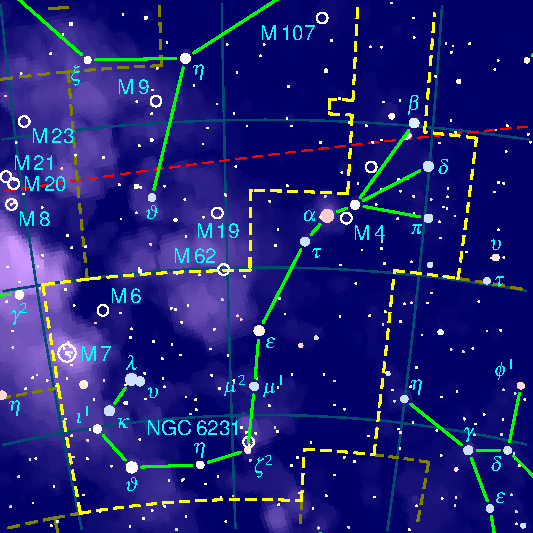
\includegraphics[scale=0.8]{sco}}
\caption{Das Sternbild Skorpion.  (Karte auf 80\,\% verkleinert.)}
\label{fig:scorpion}
\end{figure}
\fi

\medskip Man kann nun dieses kleine Skript in der Datei \verb|sco.pp3|
speichern und
\begin{verbatim}
pp3 sco.pp3
latex sco
dvips sco
\end{verbatim}
aufrufen.  \ifppthreecolour Die sich ergebene Karte ist in
Abbildung~\ref{fig:scorpion} zu sehen.\par \fi Allerdings sind insbesondere die
Farben f�r einen tonersparenden Ausdruck auf einem gew�hnlichen
Schwarz/""Wei�drucker ung�nstig.  Also setzen wir sie auf Werte, die daf�r
besser geeignet sind:
\begin{lstlisting}[columns={[l]flexible},escapeinside=`']
switch colored_stars off
color stars 0 0 0`\label{lst:Sternfarbe}'
color nebulae 0 0 0     color background 1 1 1
color grid 0.5 0.5 0.5  color ecliptic 0.3 0.3 0.3
color constellation_lines 0.7 0.7 0.7  # `\slshape Linien zwischen Sternen'
color labels 0 0 0
color boundaries 0.8 0.8 0.8           # `\slshape Sternbildgrenzen'
color highlighted_boundaries 0 0 0     # `\slshape Selektiertes Sternbild, hier Skorpion'
color milky_way 0.5 0.5 0.5
\end{lstlisting}

Farben werden bei \PPthree\ in der Form >>Rot Gr�n Blau<< (RGB-Farbmodell)
eingegeben, wobei die einzelnen Werte von 0.0 bis~1.0 reichen.  >>0~0~0<< ist
also Schwarz, >>1~1~1<< Wei�, und z.\,B. >>1~1~0<< ist Gelb.

Die erste Zeile sorgt daf�r, dass alle Sterne dieselbe Farbe erhalten.
Normalerweise versucht \PPthree\ n�mlich, die Originalf�rbung des Sternes
anhand seiner Spektralklasse nachzuahmen.  Nur durch diese Zeile bekommt
Zeile~\ref{lst:Sternfarbe} einen Sinn: Alle Sterne werden nun Schwarz gedruckt.

\ifppthreecolour\else
\begin{figure}
\centerline{\includegraphics[scale=0.8]{sco-grey}}
\caption{Das Sternbild Skorpion.  (Karte auf 80\,\% verkleinert.)}
\label{fig:scorpion-grey}
\end{figure}
\fi

Die restlichen Angaben sollten weitgehend selbsterkl�rend sein.  Das Ergebnis
ist also eine Karte des Skorpions in Schwarz auf Wei�\ifppthreecolour\else,
siehe Abbildung~\ref{fig:scorpion-grey}\fi.


\section{Bezeichnungen (Labels)}

Bishierhin ist die ganze Sache noch einigerma�en konventionell, sieht man mal
von der Tatsache ab, dass \PPthree${}+{}$\LaTeX${}+{}$dvips Vektorgraphiken
statt Bitmaps erzeugt, was f�r viele Anwendungen bereits ein gro�er Vorteil
ist.

Es w�re jedoch schade, wenn \LaTeX\ als blo�er \pstricks-Bereitsteller
herhalten m�sste.  Stattdessen kommt es ebenso f�r alle Bezeichnungen (Labels)
zum Einsatz.  Daf�r liegen die Labels in \PPthree{}s Datendateien bereits in
\LaTeX-Form vor (z.\,B. \verb|$\phi^{1}$|).

Zus�tzlich kann man Labels aber auch ausdr�cklich im Eingabeskript setzen.  Als
erstes muss man dazu das Eingabeskript durch das Schl�sselwort
\lstinline|objects_and_labels| in zwei Teile teilen, in denen jeweils nur
bestimmte Befehle erlaubt sind.  Der erste Teil ist der schon bekannte, w�hrend
der zweite Teil Himmelsobjekte und ihre Labels l�scht, erg�nzt, ver�ndert oder
repositioniert.  In diesen zweiten Teil kann man z.\,B. schreiben
\begin{lstlisting}[numbers=none]
set_label_text SCO 21 "\\footnotesize Antares"
\end{lstlisting}
Das gibt dem Stern \Flamsteed{21}{Sco} das Label "`Antares"', au�erdem stellt
es daf�r auf eine kleinere Schrift um.  "`\Flamsteed{21}{Sco}"' ist die
astronomische Bezeichnung f�r Antares, "`21"' ist dabei die sogenannte
Flamsteed-Nummer.  F�r sehr s�dliche Sternbilder, die Herr Flamsteed von London
aus nicht sehen konnte, und sehr kleine Sterne muss man die
Henry-Draper-Katalognummern benutzen:
\begin{lstlisting}[numbers=none,{columns=[l]flexible}]
set_label_text HD 128620 "\\footnotesize Toliman"        # Alpha Centauri
\end{lstlisting}
(Das Programm \emph{Celestia}~\cite{laurel:celestia} erm�glicht es, diese
Nummern f�r einen gegebenen Stern bequem herauszufinden.)


\subsection{Labelkollision vermeiden}

Eine wichtige Funktion von \PPthree\ ist die Vermeidung von �berlappungen von
Labels mit Himmelsobjekten, Linien oder anderen Labels.  Die Herangehensweise
daf�r ist ein wenig von dem Zeilenumbruchalgorithmus von \TeX\ inspiriert:
\PPthree\ probiert die acht Positionen der Windrose um das jeweilige
Himmelsobjekt, das bezeichnet werden soll, aus, und berechnet f�r jede Position
eine Strafpunktezahl, die sich durch die verschiedenen m�glichen Arten von
�berlappungen ergibt.  Die Position, die die geringste Strafpunktezahl
aufweisen kann, wird genommen.  �bersteigen diese Strafpunkte einen bestimmten
Wert, wird das Label unterdr�ckt.

Man kann diesen automatischen Mechanismus �berstimmen durch explizite
Positionierungsangabe:
\begin{lstlisting}[numbers=none,{columns=[l]flexible}]
reposition ORI 34 E ;    # Mintaka
\end{lstlisting}
Diese Anweisung setzt das Label f�r den Stern Mintaka im Orion auf �stliche
Position (also rechts).  Die acht m�glichen Positionen werden mit den typischen
englischen Abk�rzungen der Windrose bezeichnet.

\nopagebreak Es zeigt sich, dass in der Praxis nur selten in diesen
automatischen Algorithmus zur Label-Erzeugung eingegriffen werden muss.

\subsection{Manuelle Labels}

Labels werden als einfache \LaTeX-Boxen in die Karte gedruckt.  Innerhalb
dieser Boxen kann man allerlei \LaTeX- und \pstricks-Tricksereien anwenden wie
in
\begin{lstlisting}[numbers=none,showstringspaces=false]
text "\\small Wolf 359\\hskip0.3em
      \\psdots[dotstyle=+,dotangle=45](0,0)"
     at 10.902 7.32 color 0.3 0.3 0.9333 towards NW ;
\end{lstlisting}
Dieses Kommando druckt ein kleines ,$\times$` an die Position des Sterns
Wolf~359 im L�wen und schreibt "`Wolf~359"' in einer grau-blauen Farbe oben
links daneben.

Das Kommando \lstinline|text| setzt grunds�tzlich alle benutzerdefinierten
Labels.  Es folgt der Label-Text im \LaTeX-Format.  Das Schl�sselwort
\lstinline|at| leitet die Himmelskoordinaten ein, in diesem Fall $10^{\mathrm
  h}54^{\mathrm m}7{,}2^{\mathrm s}$ Rektaszension und $+7{,}32^\circ$
Deklination.  Es folgen optional die Farbe nach \lstinline|color| und die Lage
der Box nach \lstinline|towards|.

Im obigen Beispiel ist die Lage \lstinline|NW|, also oben links; das bedeutet,
dass die rechte untere Ecke der Box genau auf den gegebenen Himmelskoordinaten
liegt.  Daher kommt das \verb|\psdots|-Makro, das das ,$\times$` erzeugt, als
\emph{letztes} in der Reihe der \LaTeX-Befehle.

\begin{figure}
  \def\psftt#1 {\psfrag{#1}[c][c]{\textsf{#1}}}
  \psftt E \psftt NE \psftt N \psftt NW \psftt W \psftt SW \psftt S \psftt SE
  \psfrag{E!}[c][c]{\textsf{E\_}}
  \psfrag{W!}[c][c]{\textsf{W\_}}
  \centerline{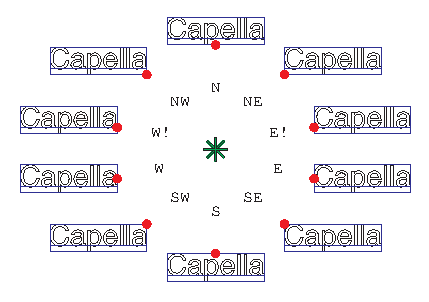
\includegraphics{pp3rose}}
  \caption{\PPthree{}s Windrose und die
    sich ergebene Ausrichtung.  Der \ifppthreecolour rote \fi Punkt liegt
    jeweils exakt auf den Himmelskoordinaten.  Dieser Parameter kommt bei
    \lstinline|towards| und \lstinline|reposition| zum Einsatz.}
  \label{fig:windrose}
\end{figure}

W�re die Lage z.\,B. "`\lstinline|towards N|"' gewesen, w�re die \emph{Mitte}
der unteren Kante der Box auf den Himmelskoordinaten zu liegen gekommen.  Die
Abbildung~\ref{fig:windrose} zeigt alle m�glichen Parameter f�r
\lstinline|towards| und welche Ausrichtung sie bewirken.

Offensichtlich werden f�r \lstinline|NW| oder \lstinline|N| die �u�ersten
Boxgrenzen und nicht die Grundlinie als Bezug benutzt.  Es ist also i.\,a.\ f�r
den Trick mit dem ,$\times$` besser, "`\lstinline|towards W_|"' zu benutzen,
denn z.\,B.  der Sternname "`\mbox{Luyten 726-8}"' hat eine Unterl�nge und
w�rde daher bei Angabe von "`\lstinline|NW|"' mitsamt dem ,$\times$` etwas nach
oben verschoben.

Wenn immer dieselben Konstrukte in den Labels vorkommen, ist es
selbstverst�ndlich m�glich und sinnvoll, daraus \LaTeX-Makros zu machen und
diese in eine benutzerdefinierte Pr�ambel (s.\,u.)\ einzubauen.  Dann werden
die Labels etwas �bersichtlicher.

\subsubsection{Gebogene Labels: Flexes}

\medskip Gerade in der N�he der Himmelspole kann es graphisch ansprechend sein,
eine Bezeichnung nicht als ordin�re Box zu setzen, sondern als Schriftzug, der
auf einem Deklinationskreis ($\mathrel{\hat=}$~Breitenkreis) entlangl�uft.  Das
\verb|pst-text|-Paket von \pstricks\ stellt einen solchen Spezialeffekt zur
Verf�gung.  Das Problem besteht also nur darin, das entsprechende Fragment des
Deklinationskreises zu finden, insbesondere seine L�nge zu bestimmen.
\PPthree\ kann sie wegen der nicht l�ngentreuen Abbildung nur absch�tzen, macht
es aber ganz ordentlich.  Das Ergebnis sind sogenannte Flex-Labels oder kurz
Flexes.  Man kann sie sehr sch�n f�r etwas l�ngere Labels, z.\,B. die
Sternbildnamen, benutzen:
\begin{lstlisting}[numbers=none]
text "Ursa Major" at 12 30 along declination towards SE ;
\end{lstlisting}
Der einzige Unterschied ist also der Schl�sselausdruck
"`\lstinline|along declination|"'.

\begin{figure}
\centerline{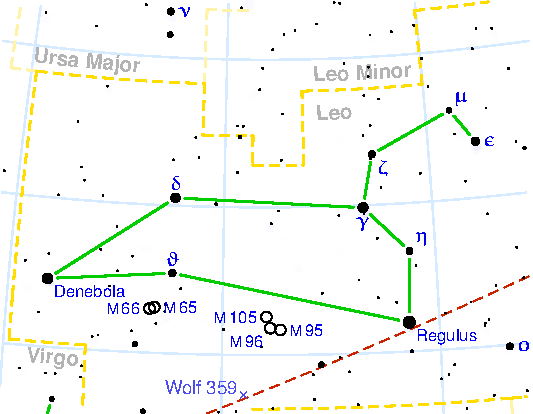
\includegraphics{leo}}
\caption{Das Sternbild L�we, mit verschiedenen Arten von Labels.}
\label{fig:leo}
\end{figure}

Als Beispiel f�r die Labels (und etwas mehr) gebe ich hier das Skript f�r das
Sternbild L�we an, dessen Ergebnis man in Abbildung~\ref{fig:leo} sieht:
\begin{lstlisting}[showstringspaces=false,escapeinside=`',extendedchars=true]
# Leo, der L�we

filename output `\texttt{leo.tex}'
filename include `\texttt{wiki.pp3}'`\label{lst:Include}'
switch eps_output on`\label{lst:EpsOutput}'

set constellation LEO
set center_rectascension 10.8 `\quad' set center_declination 20
set box_height 7 `\quad' set box_width 9

objects_and_labels`\label{lst:ObjectsAndLabels}'

reposition LEO 32 SE ;  # Regulus`\label{lst:Regulus}'
add_labels LEO 24 ;`\label{lst:AddLabels}'

text `\texttt{Leo}' at 10.55 27 along declination towards SE ;
text "Leo Minor" at 10.05 28.5 along declination towards NW ;
text "Ursa Major" at 12 30 along declination towards SE ;
text `\texttt{Virgo}' at 11.65 10 along declination towards SW ;

text "\\small Wolf 359\\hskip0.3em
    \\psdots[dotstyle=+,dotangle=45](0,0)" 
  at 10.902 7.32 color 0.3 0.3 0.9333 towards W_ ;
delete LEO 63  HD 97605 ;`\label{lst:Delete}'
\end{lstlisting}
Zeile~\ref{lst:Include} zeigt, wie man eine globale Stildatei einbinden kann:
Die Datei \verb|wiki.pp3| ist vom Aufbau her ein gew�hnliches Eingabeskript, in
dem Pr�ambel, Farben, einige Sternbildnamen wie "`Regulus"' etc.\ gesetzt
werden.  So etwas ist sehr hilfreich, wenn man eine ganze Reihe von Karten f�r
ein Projekt erzeugt.

Zeile~\ref{lst:EpsOutput} weist \PPthree\ an, direkt dvips aufzurufen, um eine
EPS-Datei zu erzeugen.  Es existiert ein analoger Befehl f�r PDF\@.

In Zeile~\ref{lst:ObjectsAndLabels} wird der zweite Teil eingel�utet, in dem
Objekte und Labels eingestellt werden: Zeile~\ref{lst:Regulus} zieht den Namen
"`Regulus"' von der gestrichelten Ekliptiklinie weg, auf die \PPthree\ ihn
sonst gesetzt h�tte.  Die Ekliptik nimmt bislang leider noch nicht an dem oben
erw�hnten Strafpunkte-Schema teil.

Zeile~\ref{lst:AddLabels} f�gt das Label von \Flamsteed{24}{Leo}
($\equiv\mathrm{\mu\,Leo}$) ein, das \PPthree\ standardm��ig unterdr�ckt h�tte,
weil der Stern zu schwach ist.  Zeile~\ref{lst:Delete} schlie�lich macht etwas
dazu gegens�tzliches: Da \Flamsteed{63}{Leo} und HD\,97605 dem Schriftzug
"`Wolf~359"' gef�hrlich nahe k�men, werden beide einfach aus der Karte
gel�scht.  Alternativ k�nnte man mit dem \verb|\colorbox|-Befehl den Schriftzug
auf einen wei�en Hintergrund setzen.

\subsection{Koordinaten-Labels}

Manchmal besteht der Wunsch, die Gitterlinien des Koordinatensystems mit
automatisch generierten Labels zu beschriften.  Das k�nnen Befehle wie
\begin{lstlisting}
text "$#3$" at 0 20 along declination tics rectascension 1 towards N ;
text "$#5$" at 11 0 along declination tics declination 10 towards S ;
\end{lstlisting}
leisten.  Die \lstinline|tics|-Option sorgt f�r eine Vervielf�ltigung des
Labels mit der angegebenen Schrittweite.  In der ersten Zeile wird in Richtung
aufsteigender Rektaszension mit der Schrittweite~$1^{\mathrm h}$
vervielf�ltigt.  Da es mit dem Punkt $(0^{\mathrm h},20^\circ)$ losgeht, wird
also der $20^\circ$-Deklinationskreis beschriftet.

Die zweite Zeile macht das analog f�r den $11^{\mathrm
  h}$-Rektaszensions-Kreis.

Im Label selber kann man folgende Platzhalter benutzen: \verb|#1| ist die
Rektaszension, \verb|#2| die Deklination.  \verb|#3| sind die vollen Stunden
der Rektaszension, \verb|#4| die vollen Minuten.  Damit lassen sich Dinge wie
$11^{\mathrm h}20^{\mathrm m}$ realisieren.  \verb|#5| ist die auf eine ganze
Zahl gerundete Deklination mit Vorzeichen, z.\,B.~"`$+20$"'.

\subsection{\LaTeX-Pr�ambel}

Es ist m�glich, \PPthree\ eine \LaTeX-Pr�ambel zu �bergeben, die dann f�r die
Erstellung der Karte benutzt wird.  So kann man eigene Stile realisieren und
insbesondere f�r typographische Konsistenz zwischen den Karten und dem
Dokument, in das die Karten eingef�gt werden sollen, sorgen.  Die bereits
erw�hnte Datei \verb|wiki.pp3| des L�we-Beispiels enth�lt z.\,B.
\begin{lstlisting}[numbers=none,escapeinside=`']
filename latex_preamble `\texttt{wiki.tex}'
\end{lstlisting}

\PPthree{}s \LaTeX-Dateien benutzen einige Hooks, in die man sich einh�ngen
kann, um globale Ver�nderungen vorzunehmen.  Die Datei \verb|wiki.tex| (die
somit auch f�r Abbildung~\ref{fig:leo} zum Einsatz kam) sieht beispielsweise so
aus:
\begin{lstlisting}[language={[LaTeX]TeX},escapeinside=`']
\usepackage[T1]{fontenc}
\usepackage{eulervm}
\renewcommand*{\sfdefault}{phv}
\usepackage{relsize}
\renewcommand{\Messier}[1]{\footnotesize{\smaller M}\,#1}`\label{lst:Messier}'
\renewcommand{\NGC}[1]{\footnotesize{\smaller NGC}\,#1}`\label{lst:NGC}'
\renewcommand{\IC}[1]{\footnotesize{\smaller IC}\,#1}`\label{lst:IC}'
\renewcommand{\FlexLabel}[1]{{\bfseries #1}}`\label{lst:FlexLabel}'
\AtBeginDocument{\sffamily\boldmath}
\end{lstlisting}
Dabei sind \lstinline|\Messier|, \lstinline|\NGC|, \lstinline|\IC| und
\lstinline|\FlexLabel| in den Zeilen~\ref{lst:Messier}--\ref{lst:FlexLabel}
einige jener Hooks.  Ihnen wird im
Parameter~\lstinline[language={[LaTeX]TeX}]|#1| die Katalognummer bzw.\ der
Label-Text �bergeben.  In diesem Beispiel sorgen sie daf�r, da� Nebel-Label
klein und Katalogk�rzel sogar noch etwas kleiner gedruckt werden.  Au�erdem
werden alle Flexes halbfett.

Im aktuellen \PPthree{} existieren f�nf weitere fest eingebaute Hooks.  Da
letztlich alles zu \LaTeX\ wird, kann man sich nat�rlich auch eigene Hooks
definieren.

\section{Interna}

\PPthree\ ist als Programm ein bunter Haufen aus vielen Einzelmodulen, allein
schon, weil eine Sternkarte aus vielen Arten von Objekten besteht.  Ich m�chte
ein paar Dinge herausgreifen und etwas n�her erl�utern.

\subsection{Datenbanken}

\PPthree\ baut auf eigenen, recht kleinen Datenbanken auf.  Sie liegen allesamt
als Textdateien vor.  Es werden vier externe Datenkompilationen benutzt: der
BSC (Sterne), der NGC/IC (Nebel), der ``Catalogue of Constellation Boundary
Data'' (Sternbildgrenzen) und das Himmels-Panorama~\cite{mellinger}
(Milchstra�e).  Bei den Sternbild-Linien habe ich die traditionellen Figuren,
die mir am besten gefielen, benutzt.

Die Originaldaten sind nicht Teil der Distribution.  F�r alle vier F�lle habe
ich jeweils ein kleines Programm geschrieben, das die u.\,U. bin�ren Daten in
Textdaten umwandelt, auf die relevanten Felder reduziert und eventuell noch in
anderer Weise aufbereitet.  Diese ``Digesters'' sind im CVS-Baum verf�gbar,
aber nicht Teil der Distribution.  Es ist ziemlich einfach, \PPthree{}s Formate
selbst zu erzeugen.

%% Es war mir �brigens nicht immer m�glich, die Lizenzbestimmungen f�r die
%% Original-Datenbanken, die f�r \PPthree\ aufbereitet wurden, in Erfahrung zu
%% bringen.  Angesichts der Art und Weise, wie diese Daten verteilt werden (und
%% insbesondere anderen Verteilungen einverleibt sind), bin ich dann von freier
%% Software ausgegangen.  Wo es ging, habe ich die freundliche Genehmigung des
%% Autors eingeholt.  Und in der Distribution werden alle Quellen genannt, so
%% genau ich es konnte.

\subsection{Kartenwurf}

\PPthree\ ist so aufgebaut, dass verschiedene Projektionen unterst�tzt werden
k�nnen, aber es ist de~facto nur eine einzige realisiert, n�mlich die
�quidistante azimutale Projektion.  Sie stellt einen Kompromiss zwischen
Winkel- und Fl�chentreue dar und ist in der Astronomie sehr beliebt.  \PPthree\ 
dreht das Zentrum jeder Karte in den Zenit der Projektion (Punkt geringster
Verzerrung) und kann daher immer die bestm�gliche Abbildung bieten.

\subsection{Milchstra�e}

Die Milchstra�e wird gezeichnet, indem eine Panorama-Bitmap~\cite{mellinger} in
Himmelskoordinaten\penalty10000--""Grauwert-Paare umgewandelt wurde, und dann
\PS-Kreise gezeichnet werden, die gerade so klein sind, dass garantiert keine
L�cken entstehen.

Das f�hrt bei zu gro�er Vergr��erung oder hochauf"|l�sender Ausgabe nat�rlich
zu Pixel-Effekten, aber f�r typische Ansichten ist das Ergebnis bei richtiger
Farbwahl ausgesprochen h�bsch, zumal wenn man bedenkt, dass es sich immer noch
um Vektordaten handelt.  Als Seiteneffekt entstehen kleine H�fe um die sehr
hellen Sterne, aber das ist eher ein nettes Feature als ein Bug.

F�r starke Vergr��erungen kann man nat�rlich noch hochauf"|l�sendere
Milchstra�enbitmaps f�r \PPthree\ aufbereiten.  Allerdings lassen sich die f�r
gr��ere Himmelsausschnitte nicht mehr verwenden, weil dann \TeX{}s Speicher
�berl�uft.  Schon jetzt ist es ratsam, f�r die Milchstra�e den Hauptspeicher
von \TeX\ auf den implementationsspezifischen Maximalwert zu setzen.


\subsection{Label-Abmessungen}

Damit \PPthree\ �berlappungen von Labels erkennen kann, muss es wissen, wie
gro� sie sind.  Daf�r wird eine Datei namens \verb|labeldimens.dat| gelesen,
die alle Label-Abmessungen enth�lt.  Da diese Datei erstmal nicht existiert und
der Benutzer ja beliebige Labels hinzuf�gen kann, erzeugt \PPthree\ f�r alle
unbekannten Labels eine tempor�re \LaTeX-Datei, die durch \LaTeX\ geschickt
wird und als Ergebnis statt einer DVI-Datei alle Label-Abmessungen an \PPthree\ 
zur�ckgibt.  Diese werden dann f�r zuk�nftige Durchl�ufe in
\verb|labeldimens.dat| gespeichert.

Die aktuell eingestellte \LaTeX-Pr�ambel kommt nat�rlich auch bei der
Berechnung der Label-Abmessungen zum Einsatz.

Wenn man die globale Font-Konfiguration in irgendeiner Weise ver�ndert, muss
man die Datei \verb|labeldimens.dat| im aktuellen Verzeichnis l�schen, um eine
Neuberechnung zu erzwingen.


\section{Originaldokumentation von \PPthree}

Es w�rde den Rahmen dieses Artikels sprengen, alle m�glichen Kommandos, die in
einer Skriptdatei benutzt werden k�nnen, aufzulisten.  Es existieren zahlreiche
Einstellm�glichkeiten f�r die Karte selber, die darzustellenden Objekte, die
Labels, die Strafpunkteberechnung, die Farben, die verschiedenen Hilfslinien
und noch mehr.\footnote{Insgesamt 14 Top-Level-Schl�sselworte, kombinierbar mit
  48 weiteren Schl�sselworten.}

Der C\texttt{++}-Quellcode von \PPthree\ ist in CWEB~\cite{Knuth_Levy2001}
geschrieben und daher sehr gut dokumentiert.  Eine umfassende Beschreibung des
Formates der Eingabeskripte findet sich auf den ersten Seiten des ge\TeX{}ten
Quellcodes, der als PDF auch von \PPthree{}s Homepage heruntergeladen werden
kann.  Leider existiert keine eigenst�ndige Bedienungsanleitung oder ein
Tutorial, wenigstens aber eine (fast vollst�ndige) Referenzkarte.

\subsection{Wikipedia-Beispielskripte}

Quasi als Entsch�digung daf�r sind viele Beispiele f�r Eingabeskripte Teil der
Distribution von \PPthree.  Es handelt sich dabei um die Originalskripte, die
bei der Erstellung der Sternbild-Karten des
Wikipedia-Projektes~\cite{wikipedia} zum Einsatz kamen.
        
\PPthree\ zeichnet f�r nahezu alle Sternkarten der englischen Ausgabe dieser
Internet-Enzyklop�die verantwortlich, und hat sich dabei bew�hrt, auch, was den
erforderlichen Arbeitseinsatz angeht: Die meisten Skripte sind eher noch
einfacher als das L�we-Beispiel von vorhin.  Zusammen mit einem kleinen
Gimp-Skript \cite{Gimp} lassen sich sogar die endg�ltigen Bitmap-Karten per
Makefile im Stapelbetrieb erstellen.


\section{Ausblick}

Folgende Erweiterungen von \PPthree\ k�nnten sich als n�tzlich erweisen:
\begin{itemize}
\item Ein Ephemeridenmodul, das die Darstellung von Sonne, Mond, Planeten etc.\ 
  in Abh�ngigkeit vom Datum zul�sst.  (Es w�rde interessant, die Mondphasen mit
  \pstricks\ nachzuempfinden.)
\item Mehr Kartenprojektionen, insbesondere eine echte winkeltreue.
\item Die Ekliptik und die Gitterlinien in das Strafpunkte-Schema aufnehmen;
  sehr kleine Sterne, die sich mit Labels �berlappen, automatisch entfernen.
\item Intern \PPthree\ auch f�r sehr gro�e Datenbanken fitmachen.
\item Die Auf"|l�sung der Milchstra�e dynamisch so w�hlen, dass trotz extrem
  genauen Milchstra�endaten \TeX{}s Speicher nicht �berl�uft; eventuell auf
  Konturdaten umstellen.
%% \item Kl�ren, ob
%%   \texttt{pdftricks}\,\cite{radhakrishnan:pdftricks}${}+{}$pdf\TeX\ besser
%%   geeignet ist, um PDFs zu erzeugen.
\item Kleine Bitmaps aus allen Labels machen, um die
  Unterschneidungs"=Parameter auszumessen.  Das "`$\eta$"' in
  Abbildung~\ref{fig:leo} beispielsweise sollte ein wenig n�her an den Stern
  ger�ckt werden.
\end{itemize}

\section{Zusammenfassung}

Das Programm \PPthree\ ist gut geeignet, um Sternkarten f�r
popul�rwissenschaftliche Zwecke zu erzeugen.  Auch das Erstellen einer ganzen
Serie von Sternkarten ist relativ bequem m�glich.  Die meisten Labels werden
automatisch erzeugt und positioniert.  In manuellen Labels stehen alle in einer
horizontalen Box erlaubten \LaTeX-Befehle zur Verf�gung.  Das Layout l�sst sich
in vielf�ltiger Weise beeinflussen, und insbesondere sind nachtr�gliche
Karten-�bergreifende Stil�nderungen kein Problem.

Die Schw�chen sind die spartanische Dokumentation, das wenig intuitive und
etwas zerbrechliche Eingabeformat und der u.\,U. recht gro�e Ressourcenhunger.

Die komplette \PPthree-Distribution steht unter einer Freie-Software-Lizenz.

\bibliography{dtk_pp3}

\endinput

%%% Local Variables: 
%%% mode: latex
%%% TeX-master: "dtk"
%%% End: 

% LocalWords:  page morecomment numbers left numberstyle keywords filename set
% LocalWords:  color switch off penalty objects and labels delete add label faq
% LocalWords:  reposition text along towards basicstyle fontadjust columns Ciel
% LocalWords:  string stringstyle style Torsten Bronger Public Domain Cartes
% LocalWords:  pdf output sco tex constellation center rectascension box height
% LocalWords:  declination width scale colored stars nebulae background grid
% LocalWords:  ecliptic lines boundaries highlighted milky way none Flexes Flex
% LocalWords:  psdots dotstyle dotangle small Ursa leo Bright Catalogue NGC Him
% LocalWords:  Digesters winkel mels ten l�sendere language LaTeX TeX phv Local
% LocalWords:  mode latex master dtk End showstringspaces false hskip BSC grad
% LocalWords:  Boundary l�sung escapeinside booktabs graphicx listings textcomp
% LocalWords:  dass m�sste muss l�sst belowskip �nderung extendedchars true eps
% LocalWords:  include wiki Minor Virgo preamble Level rose tics draft zul�sst
% LocalWords:  grey

%
%
\end{document}%%%%%%%%%%%%%%%%%%%%%%%%%%%%%%%%%%%%%%%%%%%%%%%%%%%%%%%%%%%%%%%%%
%
% Local Variables: 
% mode: latex
% TeX-master: nil
% End: 
